\documentclass[aspectratio=169, xcolor=dvipsnames]{beamer}

% --- Theme Setup ---
\usetheme{Madrid}
\usecolortheme{default}

% --- Packages ---
\usepackage{graphicx}
\usepackage{xcolor}
\usepackage{booktabs}
\usepackage{hyperref}
\usepackage{adjustbox}
\usepackage{amssymb}
\usepackage{amsmath}
\usepackage{listings}
\usepackage{caption}

\lstset{
  basicstyle=\ttfamily\small,
  keywordstyle=\color{blue}\bfseries,
  stringstyle=\color{red},
  showstringspaces=false,
  breaklines=true
}

% --- Title Information ---
\title{Module 16}
\subtitle{Formal Relational Query Languages/1}
\author{Milav Dabgar}
\institute{www.milav.in}
\date{\today}

\begin{document}

% Title Slide
\begin{frame}
    \titlepage
\end{frame}

\begin{frame}{Week Recap}
    \begin{itemize}
        \item SQL Examples have been practiced for basic query structures
        \item Nested Subquery in SQL
        \item Data Modification
        \item SQL expressions for Join and Views
        \item Transactions
        \item Integrity Constraints
        \item More data types in SQL
        \item Authorization in SQL
        \item Functions and Procedures in SQL
        \item Triggers
    \end{itemize}
\end{frame}

\begin{frame}{Module Objectives}
    \begin{itemize}
        \item To understand formal query language through relational algebra
    \end{itemize}
\end{frame}

\begin{frame}{Module Outline}
    \begin{itemize}
        \item Relational Algebra
    \end{itemize}
\end{frame}

\begin{frame}{Formal Relational Query Language}
    \begin{itemize}
        \item Relational Algebra
        \begin{itemize}
            \item Procedural and Algebra based
        \end{itemize}
        \item Tuple Relational Calculus
        \begin{itemize}
            \item Non-Procedural and Predicate Calculus based
        \end{itemize}
        \item Domain Relational Calculus
        \begin{itemize}
            \item Non-Procedural and Predicate Calculus based
        \end{itemize}
    \end{itemize}
\end{frame}

\section{Relational Algebra}
\begin{frame}
  \vfill
  \centering
  \begin{beamercolorbox}[sep=8pt,center,shadow=true,rounded=true]{title}
    \usebeamerfont{title}Relational Algebra\par%
  \end{beamercolorbox}
  \vfill
\end{frame}

\begin{frame}{Relational Algebra}
    \begin{itemize}
        \item Created by Edgar F Codd at IBM in 1970
        \item Procedural language
        \item Six basic operators:
        \begin{itemize}
            \item select: $\sigma$
            \item project: $\Pi$
            \item union: $\cup$
            \item set difference: $-$
            \item Cartesian product: $\times$
            \item rename: $\rho$
        \end{itemize}
        \item The operators take one or two relations as inputs and produce a new relation as a result
    \end{itemize}
\end{frame}

\section{Select}
\begin{frame}
  \vfill
  \centering
  \begin{beamercolorbox}[sep=8pt,center,shadow=true,rounded=true]{title}
    \usebeamerfont{title}Select\par%
  \end{beamercolorbox}
  \vfill
\end{frame}

\begin{frame}{Select Operation}
    \begin{itemize}
        \item Notation: $\sigma_p(r)$
        \item $p$ is called the selection predicate
        \item Defined as:
        \[ \sigma_p(r) = \{t \mid t \in r \text{ and } p(t)\} \]
        where $p$ is a formula in propositional calculus consisting of terms connected by: $\land$ (and), $\lor$ (or), $\lnot$ (not). Each term is one of:
        \[ \langle \text{attribute} \rangle \text{ op } \langle \text{attribute} \rangle \text{ or } \langle \text{constant} \rangle \]
        where op is one of: $=, \neq, >, \geq, <, \leq$
        \item Example of selection: 
        \[ \sigma_{\text{dept\_name} = '\text{Physics}'}(\text{instructor}) \]
    \end{itemize}
\end{frame}

\begin{frame}{Select Operation Examples}
    \begin{center}
        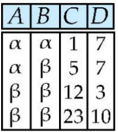
\includegraphics[width=0.6\textwidth]{../Lecture 4.1_artifacts/image_000008_8bd0c132939c9c9432fa01f7f21c841624569c388ec538d991147639c511a717.png}
    \end{center}
    \vspace{0.5em}
    \begin{center}
        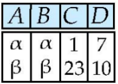
\includegraphics[width=0.6\textwidth]{../Lecture 4.1_artifacts/image_000009_dc3e0bf4c8911633b01552a93fd9e95fb1167c884db1c471e28d0d4d0c4ed4f0.png}
    \end{center}
\end{frame}

\section{Project}
\begin{frame}
  \vfill
  \centering
  \begin{beamercolorbox}[sep=8pt,center,shadow=true,rounded=true]{title}
    \usebeamerfont{title}Project\par%
  \end{beamercolorbox}
  \vfill
\end{frame}

\begin{frame}{Project Operation}
    \begin{itemize}
        \item Notation: $\Pi_{A_1, A_2, \dots, A_k}(r)$ where $A_1, A_2, \dots, A_k$ are attribute names and $r$ is a relation
        \item The result is defined as the relation of $k$ columns obtained by erasing the columns that are not listed
        \item Duplicate rows removed from result, since relations are sets
        \item Example: To eliminate the \texttt{dept\_name} attribute of \texttt{instructor}
        \[ \Pi_{\text{ID, name, salary}}(\text{instructor}) \]
    \end{itemize}
    \begin{center}
        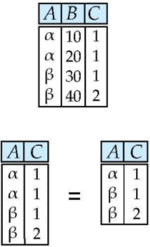
\includegraphics[width=0.6\textwidth]{../Lecture 4.1_artifacts/image_000011_6a0c098e7b31195aa84520d7039b6525ca83a024cccbf60196ff2c7fdaf2ebca.png}
    \end{center}
\end{frame}

\section{Union}
\begin{frame}
  \vfill
  \centering
  \begin{beamercolorbox}[sep=8pt,center,shadow=true,rounded=true]{title}
    \usebeamerfont{title}Union\par%
  \end{beamercolorbox}
  \vfill
\end{frame}

\begin{frame}{Union Operation}
    \begin{itemize}
        \item Notation: $r \cup s$
        \item Defined as: $r \cup s = \{t \mid t \in r \text{ or } t \in s\}$
        \item For $r \cup s$ to be valid:
        \begin{enumerate}
            \item $r, s$ must have the same arity (same number of attributes)
            \item The attribute domains must be compatible (example: 2nd column of $r$ deals with the same type of values as does the 2nd column of $s$)
        \end{enumerate}
        \item Example: to find all courses taught in the Fall 2009 semester, or in the Spring 2010 semester, or in both
    \end{itemize}
    \begin{center}
        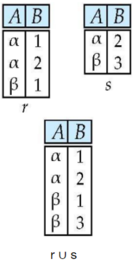
\includegraphics[width=0.9\textwidth]{../Lecture 4.1_artifacts/image_000013_7e6a5e6920b2185c32aa5d692fc71f9f03a3da861caf3bdc38dd7d032695fa8f.png}
    \end{center}
\end{frame}

\section{Difference}
\begin{frame}
  \vfill
  \centering
  \begin{beamercolorbox}[sep=8pt,center,shadow=true,rounded=true]{title}
    \usebeamerfont{title}Difference\par%
  \end{beamercolorbox}
  \vfill
\end{frame}

\begin{frame}{Difference Operation}
    \begin{itemize}
        \item Notation: $r - s$
        \item Defined as: $r - s = \{t \mid t \in r \text{ and } t \notin s\}$
        \item Set differences must be taken between compatible relations
        \begin{itemize}
            \item $r$ and $s$ must have the same arity
            \item attribute domains of $r$ and $s$ must be compatible
        \end{itemize}
        \item Example: to find all courses taught in the Fall 2009 semester, but not in the Spring 2010 semester
    \end{itemize}
    \begin{center}
        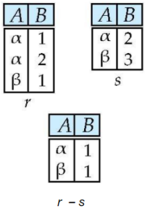
\includegraphics[width=0.9\textwidth]{../Lecture 4.1_artifacts/image_000015_c0f778ae37df2a5b1c2ee72f19aed5a2035bccb52d2b02a8f0ed4db2b82ad234.png}
    \end{center}
\end{frame}

\section{Intersection}
\begin{frame}
  \vfill
  \centering
  \begin{beamercolorbox}[sep=8pt,center,shadow=true,rounded=true]{title}
    \usebeamerfont{title}Intersection\par%
  \end{beamercolorbox}
  \vfill
\end{frame}

\begin{frame}{Intersection Operation}
    \begin{itemize}
        \item Notation: $r \cap s$
        \item Defined as: $r \cap s = \{t \mid t \in r \text{ and } t \in s\}$
        \item Assume: $r, s$ have the same arity, attributes of $r$ and $s$ are compatible
        \item Note: $r \cap s = r - (r - s)$
    \end{itemize}
    \begin{center}
        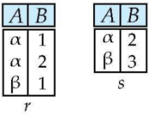
\includegraphics[width=0.45\textwidth]{../Lecture 4.1_artifacts/image_000017_90c395d58973a3011baf8e41acd9df71b9d3df7ce99b2f348bbc15e1d321df5e.png}
        \hfill
        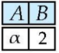
\includegraphics[width=0.45\textwidth]{../Lecture 4.1_artifacts/image_000018_93a3933842ea1fa6829d8ade18a27923860180dab714b4a4165c3de635462234.png}
    \end{center}
\end{frame}

\section{Cartesian Product}
\begin{frame}
  \vfill
  \centering
  \begin{beamercolorbox}[sep=8pt,center,shadow=true,rounded=true]{title}
    \usebeamerfont{title}Cartesian Product\par%
  \end{beamercolorbox}
  \vfill
\end{frame}

\begin{frame}{Cartesian-Product Operation}
    \begin{itemize}
        \item Notation: $r \times s$
        \item Defined as:
        \[ r \times s = \{t q \mid t \in r \text{ and } q \in s\} \]
        \item Assume that attributes of $r(R)$ and $s(S)$ are disjoint. (That is, $R \cap S = \emptyset$)
        \item If attributes of $r(R)$ and $s(S)$ are not disjoint, then renaming must be used
    \end{itemize}
    \begin{center}
        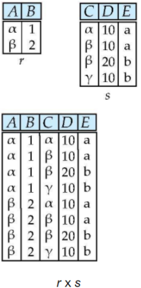
\includegraphics[width=0.6\textwidth]{../Lecture 4.1_artifacts/image_000020_39834c8affc9fb57b4befce878a5a1fa12cda74a86de3d0728c6d46caf601301.png}
    \end{center}
\end{frame}

\section{Rename}
\begin{frame}
  \vfill
  \centering
  \begin{beamercolorbox}[sep=8pt,center,shadow=true,rounded=true]{title}
    \usebeamerfont{title}Rename\par%
  \end{beamercolorbox}
  \vfill
\end{frame}

\begin{frame}{Rename Operation}
    \begin{itemize}
        \item Allows us to name, and therefore to refer to, the results of relational-algebra expressions.
        \item Allows us to refer to a relation by more than one name.
        \item Example: $\rho_X(E)$ returns the expression $E$ under the name $X$
        \item If a relational-algebra expression $E$ has arity $n$, then
        \[ \rho_{X(A_1, A_2, \dots, A_n)}(E) \]
        returns the result of expression $E$ under the name $X$, and with the attributes renamed to $A_1, A_2, \dots, A_n$.
    \end{itemize}
\end{frame}

\section{Division}
\begin{frame}
  \vfill
  \centering
  \begin{beamercolorbox}[sep=8pt,center,shadow=true,rounded=true]{title}
    \usebeamerfont{title}Division\par%
  \end{beamercolorbox}
  \vfill
\end{frame}

\begin{frame}{Division Operation}
    \begin{itemize}
        \item The division operation is applied to two relations
        \item $R(Z) \div S(X)$, where $X \subset Z$. Let $Y = Z - X$ (and hence $Z = X \cup Y$); that is, let $Y$ be the set of attributes of $R$ that are not attributes of $S$
        \item The result of DIVISION is a relation $T(Y)$ that includes a tuple $t$ if tuples $t_R$ appear in $R$ with $t_R[Y] = t$, and with $t_R[X] = t_S$ for every tuple $t_S$ in $S$.
        \item For a tuple $t$ to appear in the result $T$ of the DIVISION, the values in $t$ must appear in $R$ in combination with every tuple in $S$
        \item Division is a derived operation and can be expressed in terms of other operations:
        \[ r \div s \equiv \Pi_{R-S}(r) - \Pi_{R-S}((\Pi_{R-S}(r) \times s) - \Pi_{R-S, S}(r)) \]
    \end{itemize}
\end{frame}

\begin{frame}{Division Examples}
    \begin{center}
        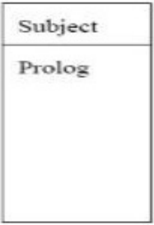
\includegraphics[width=0.45\textwidth]{../Lecture 4.1_artifacts/image_000024_420cf06f245ae4cca4614707e947c000783e1313ecd6562cc6e25469f50c4563.png}
        \hfill
        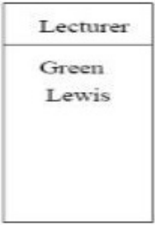
\includegraphics[width=0.45\textwidth]{../Lecture 4.1_artifacts/image_000025_6f8c738645e65586a57fe1bcd4389fa011dfbb8517333af68bfa592e18699336.png}
    \end{center}
\end{frame}

\begin{frame}{Division Examples (2)}
    \begin{center}
        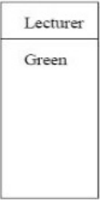
\includegraphics[width=0.3\textwidth]{../Lecture 4.1_artifacts/image_000027_2c316faaeddf57b9ceaec6bcf29b748b3bad0bb3f25ab7a04aab9cfb41d1ad79.png}
        \hfill
        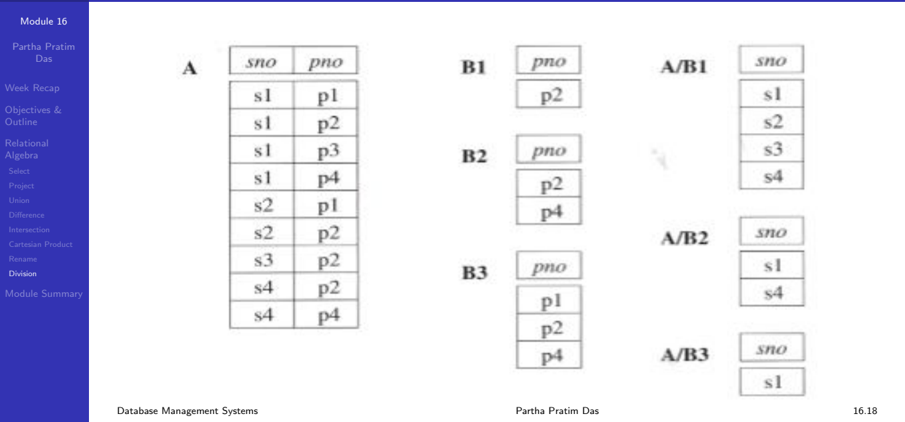
\includegraphics[width=0.6\textwidth]{../Lecture 4.1_artifacts/image_000029_daabb652c0df64782e685580632cb39fca9accc154c89b4b4a074d7ce2cd180b.png}
    \end{center}
\end{frame}

\begin{frame}{Division Examples (3)}
    \begin{center}
        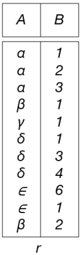
\includegraphics[width=0.45\textwidth]{../Lecture 4.1_artifacts/image_000031_a2f3aa8c48d35291a629b69175ff76d4542006a682dd71f25de6b14fa1177518.png}
        \hfill
        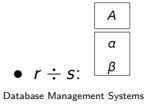
\includegraphics[width=0.45\textwidth]{../Lecture 4.1_artifacts/image_000032_c277774fa8f1038bffc31d9c5ac59588b1e3bc295c46abe0b4034a3cf56a36c8.png}
    \end{center}
    \begin{itemize}
        \item e.g. A is customer name, B is branch-name. 1 and 2 here show two specific branch-names (Find customers who have an account in all branches of the bank)
    \end{itemize}
\end{frame}

\begin{frame}{Division Example (4)}
    \begin{center}
        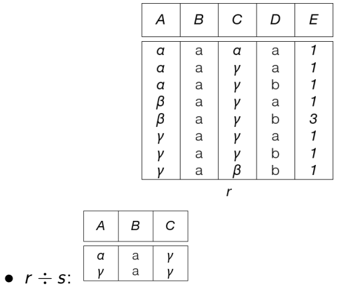
\includegraphics[width=0.45\textwidth]{../Lecture 4.1_artifacts/image_000035_f7e0c53d4904413b2e47c9899d5047057aa7b20b28933dec7bcf5d6328a4d948.png}
    \end{center}
    \begin{itemize}
        \item e.g. Students who have taken both 'a' and 'b' courses, with instructor '1'
        \item (Find students who have taken all courses given by instructor 1)
    \end{itemize}
\end{frame}

\begin{frame}{Module Summary}
    \begin{itemize}
        \item Discussed relational algebra with examples
    \end{itemize}
    \vspace{2em}
    \begin{center}
    \small \textit{Slides used in this presentation are borrowed from \url{http://db-book.com/} with kind permission of the authors.} \\
    \small \textit{Edited and new slides are marked with 'PPD'.}
    \end{center}
\end{frame}

\end{document}
